\documentclass[tikz,border=10pt]{standalone}
\usetikzlibrary{calc}
\begin{document}
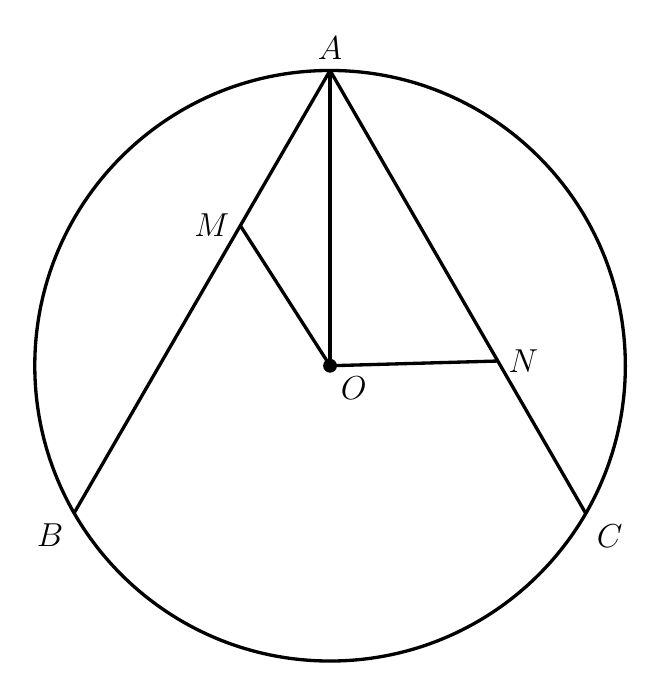
\begin{tikzpicture}[line width=1.2pt, line join=round]
% Scale s = 0.010596 cm/px (STYLE METRICS): longest side = 8 cm
% Named coordinates
\coordinate (O) at (0,0);
\coordinate (A) at (0,3.75);      % top point on circle
\coordinate (B) at (-3.25,-1.87); % lower-left on circle
\coordinate (C) at (3.25,-1.88);  % lower-right on circle
\coordinate (M) at (-1.14,1.78);  % lies on AB
\coordinate (N) at (2.13,0.06);   % on horizontal radius

% Circle centred at O, radius 354.31 px
\draw (O) circle (3.75);

% Chords from A (BC removed: not in original)
\draw (A) -- (B);
\draw (A) -- (C);

% Segments from centre
\draw (A) -- (O);   % vertical
\draw (O) -- (M);   % to point on AB
\draw (O) -- (N);   % horizontal to N

% One larger filled dot at O only
\fill (O) circle (2.5pt);

% Labels (O placed below-right)
\node[above, font=\fontsize{12.5}{15}\selectfont] at (A) {$A$};
\node[below left, font=\fontsize{12.5}{15}\selectfont] at (B) {$B$};
\node[below right, font=\fontsize{12.5}{15}\selectfont] at (C) {$C$};
\node[left, font=\fontsize{12.5}{15}\selectfont] at (M) {$M$};
\node[right, font=\fontsize{12.5}{15}\selectfont] at (N) {$N$};
\node[below right, font=\fontsize{12.5}{15}\selectfont] at (O) {$O$};
\end{tikzpicture}
\end{document}